\section{结果}

\subsection{5.1 语汇：词表把注意力压在哪几个词上}

表 \ref{tab:vocab} 给的是全部十二个词项的逐字命中。前三名是族、孝、嗣，
分别 234、167、114 次；第四名继承 82 次；再往后断崖式下滑，家族 37、名分 34、
世袭 23、祭祀 18、嫡子 17、荫 7，末两名宗族与家法各 1 次。
真正在书里被反复念的是「族」这一个字——族 234 次超过第二至第四名之和。
值得单独记一笔的是末两项：人类学写到明代宗族时最常引用的「宗族」「家法」，
在这部书里各只出现 1 次；把「宗族」当成这部叙事的组织词，是后加的概念，不是书里的词。


\begin{table}[!t]
\centering
\caption{主题词逐字命中（降序）}
\label{tab:vocab}
\small
\begin{tabular}{lr}
\toprule
词 & 命中次数 \\
\midrule
族 & 234 \\
孝 & 167 \\
嗣 & 114 \\
继承 & 82 \\
家族 & 37 \\
名分 & 34 \\
世袭 & 23 \\
祭祀 & 18 \\
嫡子 & 17 \\
荫 & 7 \\
宗族 & 1 \\
家法 & 1 \\
\bottomrule
\end{tabular}
\end{table}



\begin{figure}[!t]
\centering
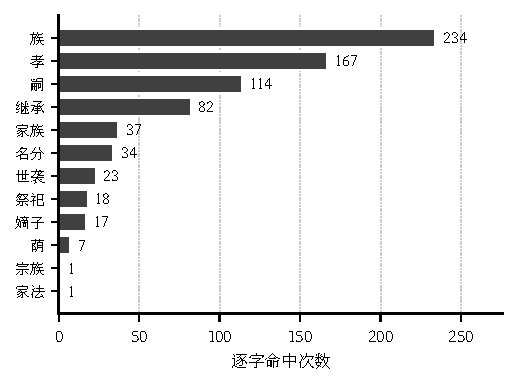
\includegraphics[width=\columnwidth]{fig_anthropology_1.pdf}
\caption{图 1 十二个主题词的逐字命中次数（降序）。注意末两项宗族与家法各 1 次。}
\label{fig:vocab}
\end{figure}


\subsection{5.2 网络形状：类别构成相对基线的位移}

130 人子图含显式边 636 条，成员在全图上的平均度数 12.6，高于（四个锚点皆为大度枢纽，这一均值是选集抬升出来的，并不表示子图内部更连通）全图平均的全图平均的 6.3。类别构成对比如表 \ref{tab:cats} 与图 \ref{fig:cats}。


\begin{table}[!t]
\centering
\caption{子图与全图的类别构成对比（括号内为边数；仅列子图或基线中占比 $\geq1\%$ 的类别）}
\label{tab:cats}
\small
\begin{tabular}{lrr}
\toprule
类别 & 子图 & 全图基线 \\
\midrule
其他 & 49.1~(312) & 39.9~(927) \\
君臣从属 & 18.2~(116) & 17.1~(397) \\
敌对冲突 & 12.6~(80) & 13.8~(321) \\
亲属 & 7.5~(48) & 8~(185) \\
同盟友党 & 5.7~(36) & 7~(162) \\
政治攻讦 & 3.6~(23) & 8.3~(193) \\
派系机构关联 & 1.7~(11) & 1.4~(33) \\
\bottomrule
\end{tabular}
\end{table}


表 \ref{tab:cats} 与图 \ref{fig:cats} 是最要紧的一张对照。
先讲不动的：亲属 7.5\%（48 条）对基线 8.0\%（185 条），只差不到一个百分点；
婚姻姻亲 0.2\%（1 条）对 0.2\%（4 条），寄基线里都排在最末。
再讲动的：未归类的「其他」由 39.9\%（927 条）抬到 49.1\%（312 条）；
政治攻讦由 8.3\%（193 条）掉到 3.6\%（23 条）；师生同门 0.5\%（3 条）对 2.7\%（63 条）。


\begin{figure}[!t]
\centering
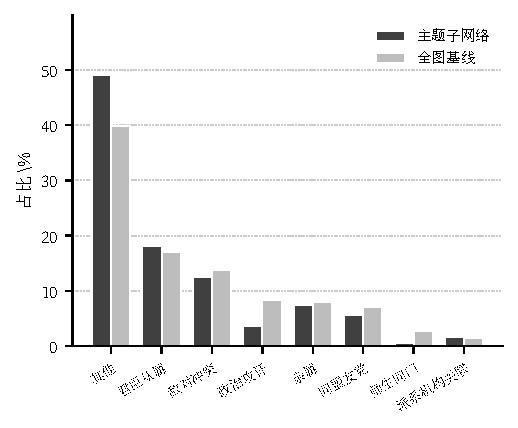
\includegraphics[width=\columnwidth]{fig_anthropology_2.pdf}
\caption{图 2 四个锚点的自我网络（子图）与全图基线在关系类别上的占比对照
（仅列子图或基线中占比不小于百分之一的类别）。横轴为类别，纵轴为占比。}
\label{fig:cats}
\end{figure}


把这两处合起来读，本篇的结果是反直觉的。母题在词汇侧压得极重
（族 234、孝 167、嗣 114、继承 82），可一旦落到关系上，亲缘这一类比全图还稍微低一点：
亲属 7.5 对 8.0，同盟友党 5.7 对 7.0，师生同门 0.5 对 2.7，全线不升反降。
留在子图顶上的仍是君臣从属（18.2，116 条）与敌对冲突（12.6，80 条）两项，
它们和基线里的位次（17.1、13.8）几乎一模一样。换句话说，这部叙事写「家国同构」时，
用的是宫廷里的君臣框架去套继承危机，而不是用乡族的亲缘框架去套朝廷；
「家」是被借来的比喻，不是被画出来的网络。同时「其他」涨了九个多百分点，
说明聚焦这四个枢纽还顺手把一批没被归类的边卷了进来——聚焦没有换来更好的编码分辨率。

\subsection{5.3 主题事件的时间分布}

图 \ref{fig:events} 只有三根等等高的柱子：1404 年、1581 年、1601 年，
各一件。这三件话题事件分别是立储之议定朱高炽为太子、争国本开端、争国本结束——
一个完整争议的起与止，外加一次更早的立储。更有信息量的是这个数量本身：
贯穿全书的继承母题，在结构化抽取里只留下三件带年份的事件、零处地点。
继承争议在书中是以人物面孔（朱棣、朱由检、朱允炆、方孝孺）被记住的，
不是以年份被记住的；这一点直接写进第 6 节的 L7。
与之对照，表 \ref{tab:anchors} 里朱元璋出场 41 章（全书 41 章）、87 度，
朱棣 113 度 / 25 章，朱由检 67 / 19 章，方孝孺 15 / 6 章——
这套语法的承载者是人物，不是年表。


\begin{figure}[!t]
\centering
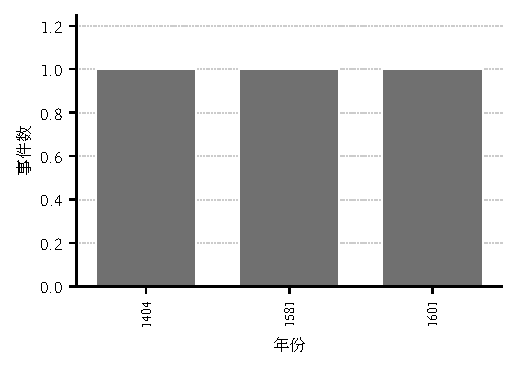
\includegraphics[width=\columnwidth]{fig_anthropology_3.pdf}
\caption{图 3 仅有的三件带年份的主题事件：1404、1581、1601 各 1 件。}
\label{fig:events}
\end{figure}


\subsection{5.4 热度与中心性}

叙事热度（出场章节数）与网络中心性（度数）的 Spearman 秩相关为 $\rho=0.871$。这一项是本篇与「热度不等于中心性」那类警告相反的一例：
在这部叙事里，出场章节数与度数近乎同一个排布，朱棣 113 度 / 25 章、
朱元璋 41 章 / 87 度两条线互相印证。也就是说，「家国同构」不是某个时期的热门专题，
而是从开篇铺到结尾的骨架——凡是被反复写到的人，正是被反复连到别人的人。

\subsection{5.5 一个不成立的结果，作为边界}

这一节本该报一个成立的结果，实测却反过来。若「家国同构」在书中真是亲缘主导，
那么以四个核心人物为锚点圈出的这批人，亲缘与婚姻边应当明显抬起、君臣边应当下沉。
实测：亲属 7.5\%（48 条）对基线 8.0\%（185 条），基本持平；
婚姻姻亲 0.2\%（1 条）对 0.2\%（4 条），同样持平；
君臣从属不但没降，还由 17.1\% 升到 18.2\%。母题词表里占首位的「族」，
换到边上并没有变成一片亲属网。这个不成立的结果比成立的结果更有用：
它提示「家国同构」是叙述者借来组织材料的比喻框架，
书里真正被连成网络的，始终是君臣、敌我与同朝这几类政治关系；
亲缘只是给这些关系提供了一套叫得出口的称谓。

以上各项均可在 \texttt{.dump/}\_stats\_anthropology.json 中逐项回溯；把任一项换成别的子集口径，位移的方向未必保持——这本身就是第 6 节要讨论的内容。
